\section{Pyramidal Neuron}
\label{sec:dendrite}
The most abundant of all neuron types in the neocortex is the pyramidal neuron. The pyramidal neuron is unique to the cerebral cortex and can be found in all layers except the first and represent between 70-85\% of the total population in any cortical area. It has therefore been seen as the principle neuron of the cerebral cortex \cite{PyramidalPop}. As the name indicates, the cell body, or \textit{soma}, of the pyramidal neuron has a pyramidal shape, which can be seen in \autoref{fig:pyramidal}.


\begin{figure}[ht!]
    \centering
    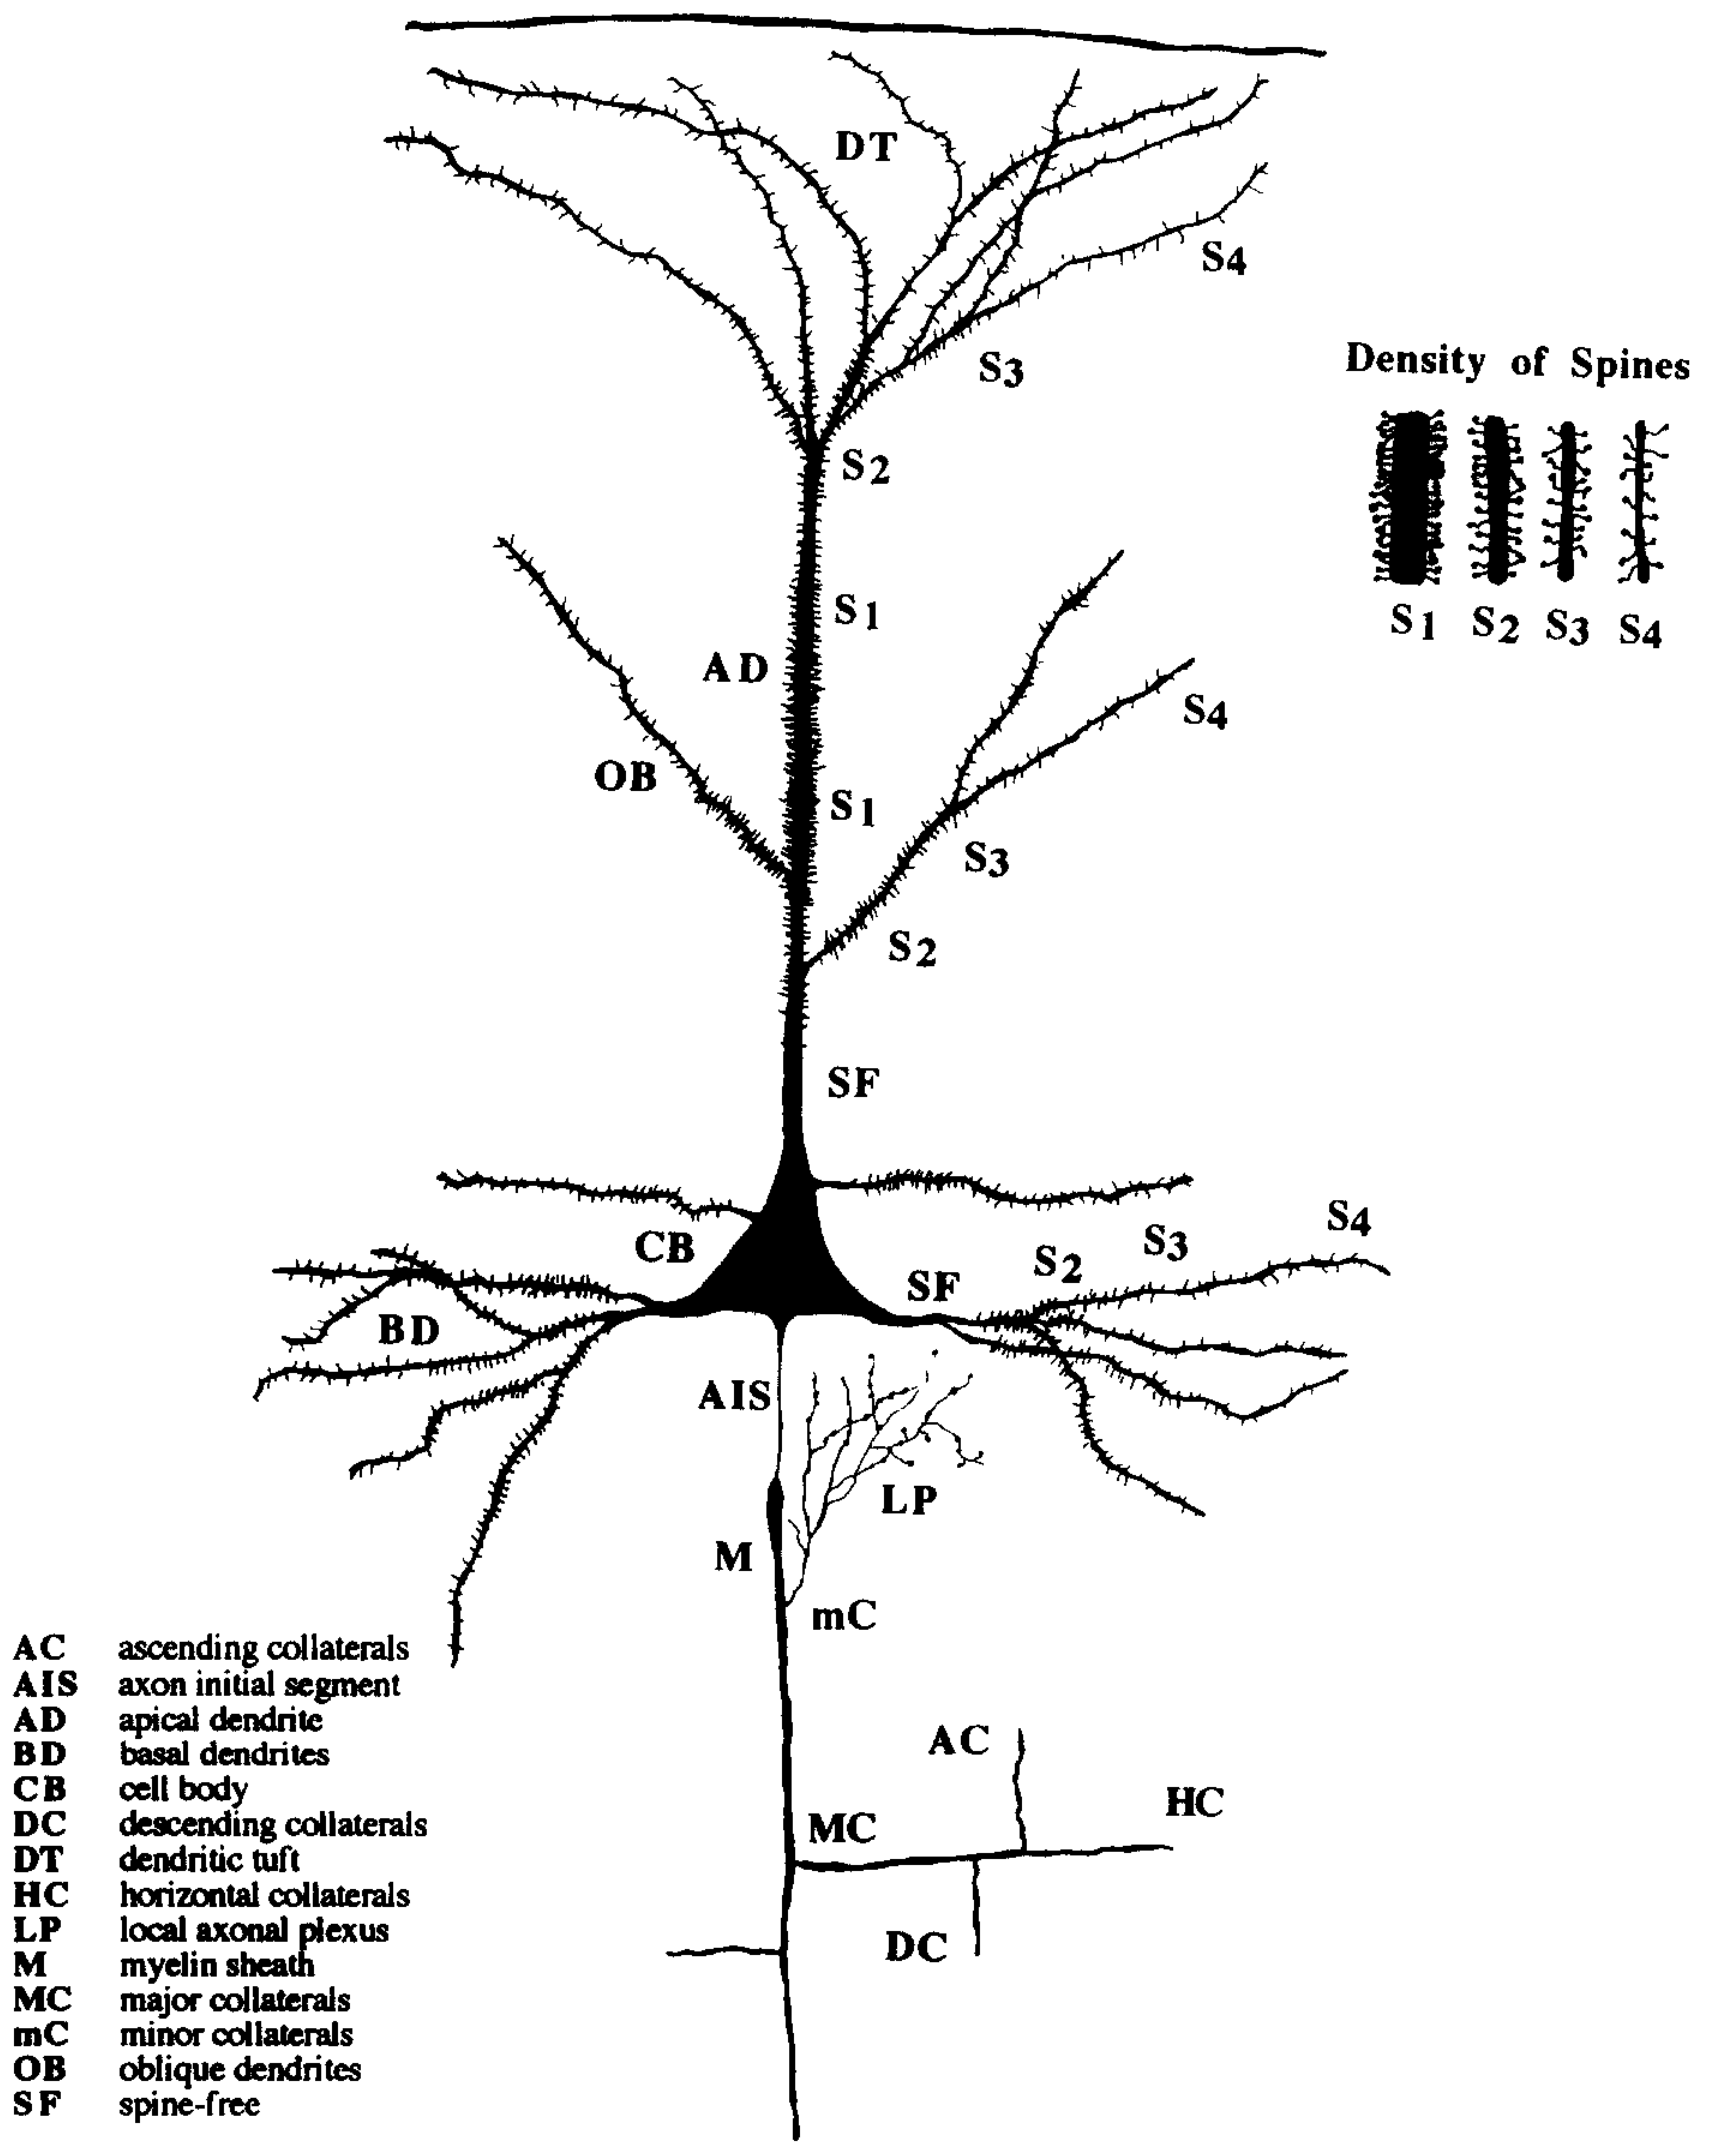
\includegraphics[scale=.3]{appendix/neuroscience/figures/PyramidalNeuron.png}
    \caption{\cite{PyramidalPop} A sketch of a stereotypical pyramidal neuron, with a apical dendrite branching out from the apex of the soma, the basal dendrites extends out in the horizontal direction and the axon is descending from the soma.}
    \label{fig:pyramidal}
\end{figure}


\subsection{Dendrites, Synapses and Axons}
The \textit{dendrites} are the input branches of a neuron, which is either able to excite or inhibit the neuron based on the neurotransmitter it receives on its \textit{synapses}. The synapses are the connections between the output branches, or \textit{axons}, and the dendrites, that allows electrical or chemical signal to be transmitted. An axon is the main output branch of the neuron, and is able to transport the signal, or action potential, to its synapses. In the dendrites the input signals are integrated, which in turn changes the state of the neuron if a complex set of conditions are met. Firstly, the integrated signal at a spatial position on the dendrite branch needs to exceed a threshold. This threshold is dynamic as the integrated signal needs to be stronger if its further away from the soma. The second condition that needs to be met is the timing of the synaptic conductances that occur at the integration zone \cite{PyramidalNeuron}. The dendrites can be classified into three zones, the \textit{basal}, \textit{proximal} and \textit{distal} zone. The basal zone contains the basal dendrites that extend along the horizontal axis and connect to neighbouring neurons in the cortical column. The apical dendrite can be divided into two parts, a proximal zone, closer to the soma, and the distal zone which is further away. In the distal zone the amplitude of the integrated signal needs to be higher in order to effect the cell state, due to the longer travel distance. The pyramidal neuron is believed to act as a coincidence detector as its been shown to respond best to simultaneous stimulation in distal and proximal areas of the apical dendrite \cite{PyramidalNeuron}. Another important feature of the pyramidal neurons is its ability to adapt to change in the temporal input patterns. It able to change functionality due to synaptic plasticity, which is ability to change the strength of the synaptic connection between neurons \cite{PyramidalNeuron}. As explained in the previous section, the strength of the synaptic connections alters with long-term potentiation or long-term depression.